\section{Linear Regression}

\subsection{Basic approaches}
\subsubsection{Maximum likelihood}
\begin{itemize}
	\item Given a dataset $D=(\bm{x}_1, \bm{x}_2, ..., \bm{x}_N)$ of $N$ independent observations
	\item The likelihood of the dataset given the model parameters $\bm{w}$ is specified as $p(D|\bm{w})$
	\item \textit{Maximum likelihood estimation}: the most likely ``explanation'' of $D$ is $\bm{w}_{\text{ML}}$:
	$$\bm{w}_{\text{ML}} = \arg\max_{\bm{w}} p(D|\bm{w})$$
	\item Using the i.i.d. assumption, we can state $p(D|\bm{w}) = \prod\limits_{n=1}^{N} p(\bm{x}_n|\bm{w})$
	\item For preventing numerical overflow and mostly simplifying the derivation, we can take the logarithm $\log p(D|\bm{w})$
	\item Maximum where $\frac{\partial}{\partial \bm{w}}\log p(D|\bm{w}) = 0$
	\item We can check whether our estimation is biased by comparing the expected result by the distribution parameters: $$\mathbb{E}\left[\sigma_{ML}^{2}\right] = \mathbb{E}\left[\frac{1}{N}\sum\limits_{i=1}^{N}\left(x_i - \frac{1}{N}\sum_{n=1}^{N} x_n\right)^2\right] = \frac{N-1}{N} \sigma^2 \implies \text{biased estimator}$$
\end{itemize}
\subsubsection{Maximum a posteriori}
\begin{itemize}
	\item Choose the most probable model parameters $\bm{w}$ given data $D$:
	$$\bm{w}_{\text{MAP}} = \arg\max_{\bm{w}} p(\bm{w}|D)$$
	\item By applying the Bayes rule (and log), we get:
	$$\bm{w}_{\text{MAP}} = \arg\max_{\bm{w}} \log p(D|\bm{w}) + \log p(\bm{w}) - \log p(D)$$
	\item We can drop the evidence as it is independent of $\bm{w}$
\end{itemize}
\subsubsection{Bayesian approach}
\begin{itemize}
	\item Frequentist approaches only consider point estimates without taking the uncertainty of the prediction into account
	\item Given a prior belief over $\bm{w}$, we are interested in the posterior distribution (not only maximum!)
	\item The predictive distribution for a new data point $\bm{x}'$ is therefore 
	$$p(t'|\bm{x}',D) = \int p(t'| \bm{x}', \bm{w}) \cdot p(\bm{w}|D) d\bm{w}$$
	\item Thus, we also consider our uncertainty when predicting
	\item However, we need to compute the evidence for that which is mostly quite hard (prefer less complex models)
\end{itemize}
\subsection{Model selection for supervised learning}
\begin{itemize}
	\item Model selection comes with two main questions:
	\begin{enumerate}
		\item How can we estimate the performance of a model on unknown data?
		\item How can we choose the optimal hyperparameters? $\Rightarrow$ \textbf{model selection}
	\end{enumerate}
	\item Common approach for large datasets: split in train, val and test dataset
	\begin{description}
		\item[Training dataset] About 80\% of the data should be used for training. On this, we try to minimize the error/loss $L\left(y(\bm{x}_i),t_i\right)$ for $(\bm{x},t)\in D_{train}$ and find optimal parameters $\bm{w}^*$.
		\item[Validation dataset] About 10\% of the data is used for estimating the test error $L\left(y(\bm{x}_{\text{val}}, \bm{w}^*),t_{\text{val}}\right)$ for various $\bm{w}^*$ from different hyperparameters. Hence, the hyperparameters are tuned on the validation dataset.
		\item[Testing dataset] The last 10\% of the available data provides the final test of the chosen best weights and hyperparameters. This data is used to estimate the performance on unseen data, and should therefore not be used for any parameter choosing!
	\end{description}
	\item However, for a small dataset, the validation and test set is very small and, hence, very noisy $\Rightarrow$ use cross validation
\end{itemize}
\subsubsection{Cross Validation}
\begin{itemize}
	\item Split data into $K$ folds % $D=\left\{\left(x_1, t_1\right), \left(x_2, t_2\right), ..., \left(x_N, t_N\right)\right\}$
	\item If $K=N$, it is also called leave-one-out cross validation as the validation is one single data point
	\item Train the model $y$ on $K-1$ folds, and test on the remaining fold $k$ $\Rightarrow$ model $\hat{y}^{\mbox{--}k}(x)$
	\item The estimation of the prediction error is the mean validation error over all folds. With the index function $\kappa:\left\{1,...,N\right\}\mapsto\left\{1,...,K\right\}$ (mapping data point to corresponding fold where it is used for validation), we get:
	$$CV(\hat{y}) = \frac{1}{N}\sum\limits_{i=1}^{N}L\left(\hat{y}^{\mbox{--}\kappa\left(i\right)}(\bm{x}_i), t_i\right)$$
	\item Task of model selection: Run cross validation for each possible parameter setting and choose the one with lowest cross validation error
	\item Task of test error estimation: after finding the best hyperparameters like $\alpha^*$, retrain model on all $K$ folds, and test this model on a held-out test set
	\item However, if test set is small, we again get a noisy estimation $\Rightarrow$ Nested cross validation
	\item Drawback of cross validation: it is computationally expensive and should therefore only be used for fast trainings/small datasets
\end{itemize}
\subsubsection{Nested Cross Validation}
\begin{itemize}
	\item Cross validation for both model selection and model performance by reusing dataset for testing
	\item General algorithm:
	\begin{enumerate}
		\item Split dataset into $M$ cross validation folds
		\item For each of these folds $m=1,...,M$:
		\begin{enumerate}
			\item Let fold $m$ be the test dataset
			\item Apply cross validation on the remaining data by splitting it into $K$ folds and find best hyperparameters $\alpha^*,\beta^*,...$
			\item Retrain the model with the best hyperparameters on all data besides the fold $m$
			\item Test the model on unseen data fold $m$ 
		\end{enumerate}
		\item The final generalization error/loss on unseen data is the mean over all $M$ folds
	\end{enumerate}
	\item For choosing the best hyperparameters $\alpha^*,\beta^*,...$, we use single cross validation on the whole dataset again without a test dataset, but record the found generalization error as estimation for unknown data, also for the new model
\end{itemize}
\begin{figure}[ht]
	\centering
	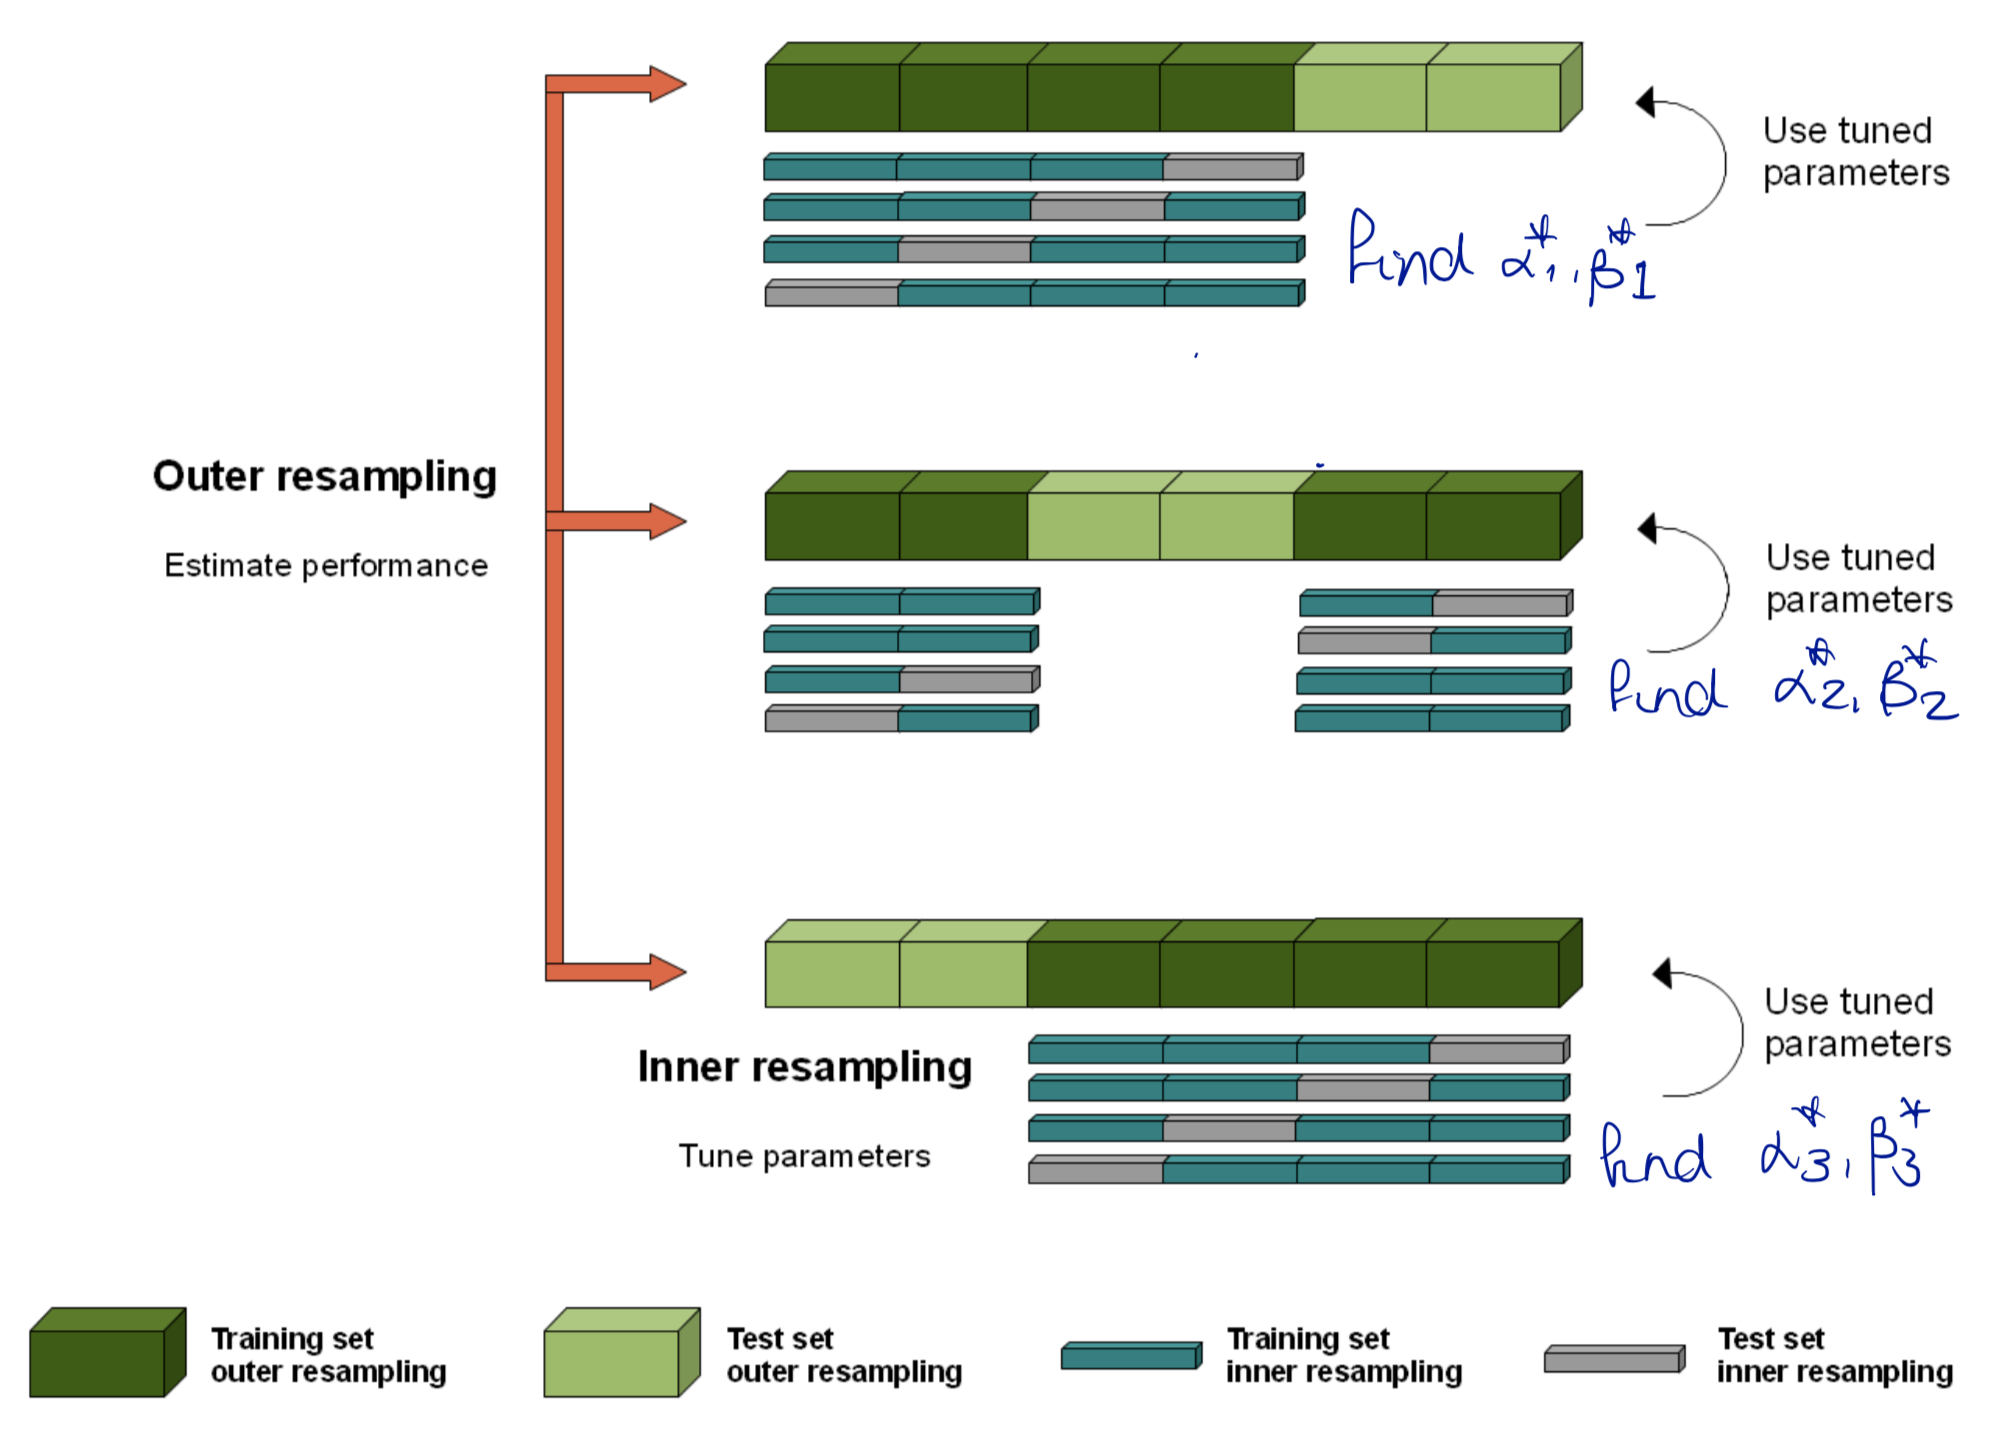
\includegraphics[width=0.5\textwidth]{figures/cross_validation_nested.png}
	\caption{Illustration of nested cross validation. The outer loop splits dataset into test and trainval parts. Within the trainval parts, we apply cross validation to find optimal hyperparameters. Those are tested on the left-out fold from the outer loop, and the mean test error of all folds is the final generalization error. Note that every outer fold can lead to different optimal hyperparameters.}
	\label{img:linear_regression_nested_cross_validation}
\end{figure}
\subsection{Bias variance decomposition}
\begin{itemize}
	\item Frequentist view on model complexity
	\item Common loss: the squared loss function, defined as $L\left(t, y\left(\bm{x}\right)\right) = \left(t - y\left(\bm{x}\right)\right)^2$
	% \item The expected loss is $\mathbb{E}\left[L\left(t, y\left(\bm{x}\right)\right)\right]=\int\int \left(t - y\left(\bm{x}\right)\right)^2 p\left(\bm{x}, t\right) \text{d}\bm{x} \text{ d}t$
	\item An optimal model of $y\left(\bm{x}\right)$ would minimize this loss which is given by $$h(\bm{x}) = \mathbb{E}\left[t|\bm{x}\right] = \int t\cdot p\left(t|\bm{x}\right) \text{d}t$$
	where the conditional distribution $p\left(t|\bm{x}\right)$ is the actual, noisy data distribution (not known!)
	\item Thus, the expected squared loss can be written as
	$$\mathbb{E}\left[L\right] = \int\underbrace{\left\{y(\bm{x}) - \mathbb{E}\left[t|\bm{x}\right]\right\}^2}_{\text{model loss}} p(\bm{x}) \text{d}\bm{x} + \int\underbrace{\left\{\mathbb{E}\left[t|\bm{x}\right] - t\right\}^2}_{\text{intrinsic noise on data}} p(\bm{x},t) \text{d}\bm{x}\text{ d}t$$
	where the first term, the model loss, depends on how different the model $y(\bm{x})$ is from the actual data distribution, and the second term arises from the intrinsic noise and represents the minimum achievable expected loss
	\item In Bayesian approach, we would model $y(\bm{x}, \bm{w})$ where the uncertainty of $\bm{w}$ is expressed in the posterior distribution
	\item However, from a frequentist viewpoint, we use multiple datasets $\mathcal{D}$ on which we train our model and get a single estimation $\bm{\hat{w}}$ for each of them. The final model is the average over this ensemble of datasets.
	\item To apply this approach, we take the model loss for a single input $\bm{x}$, and add the expected model over all datasets:
	\begin{equation*}
		\begin{split}
			\left\{y\left(\bm{x};\mathcal{D}\right) - h\left(\bm{x}\right)\right\}^2 & = \left\{y\left(\bm{x};\mathcal{D}\right) - \mathbb{E}_{\mathcal{D}}\left[y\left(\bm{x};\mathcal{D}\right)\right] + \mathbb{E}_{\mathcal{D}}\left[y\left(\bm{x};\mathcal{D}\right)\right] - h\left(\bm{x}\right)\right\}^2\\
			& = \left\{y\left(\bm{x};\mathcal{D}\right) - \mathbb{E}_{\mathcal{D}}\left[y\left(\bm{x};\mathcal{D}\right)\right]\right\}^2 + \left\{\mathbb{E}_{\mathcal{D}}\left[y\left(\bm{x};\mathcal{D}\right)\right] - h\left(\bm{x}\right)\right\}^2 \\
			& \text{\hspace{5mm} } + 2\left\{y\left(\bm{x};\mathcal{D}\right) - \mathbb{E}_{\mathcal{D}}\left[y\left(\bm{x};\mathcal{D}\right)\right]\right\}\left\{ \mathbb{E}_{\mathcal{D}}\left[y\left(\bm{x};\mathcal{D}\right)\right] - h\left(\bm{x}\right)\right\}
		\end{split}
	\end{equation*}
	\item The final model of the frequentist approach is the expected value of this loss over all datasets:
	\begin{equation*}
		\begin{split}
			\mathbb{E}_{\mathcal{D}}\left[\left\{y\left(\bm{x};\mathcal{D}\right) - h\left(\bm{x}\right)\right\}^2\right] & = \underbrace{\mathbb{E}_{\mathcal{D}}\left[\left\{y\left(\bm{x};\mathcal{D}\right) - \mathbb{E}_{\mathcal{D}}\left[y\left(\bm{x};\mathcal{D}\right)\right]\right\}^2\right]}_{\text{\textcolor{red}{variance}}} + \underbrace{\left\{\mathbb{E}_{\mathcal{D}}\left[y\left(\bm{x};\mathcal{D}\right)\right] - h(\bm{x})\right\}^2}_{\textcolor{blue}{(\text{bias})^2}}
		\end{split}
	\end{equation*}
	where the first term is the \textbf{variance} of a model trained on a single dataset compared to the average, and the second term is the loss of the average/expected model over all datasets, or rather the \textbf{bias} of the model. The third term of the original equation is eliminated as only $y(\bm{x};\mathcal{D})$ is affected by the expectation operator $\mathbb{E}_{\mathcal{D}}$, and is the same as $\mathbb{E}_{\mathcal{D}}\left[y\left(\bm{x};\mathcal{D}\right)\right]$. 
	\item Coming back to the original expected squared loss, we can decompose it into three terms:
	$$\text{expected loss} = (\text{bias})^2 + \text{variance} + \text{noise}$$
	where
	\begin{equation*}
		\begin{split}
			(\text{bias})^2 &= \int \left\{\mathbb{E}_{\mathcal{D}}\left[y\left(\bm{x};\mathcal{D}\right)\right] - h(\bm{x})\right\}^2p(\bm{x}) \text{d}\bm{x}\\
			\text{variance} &= \int \mathbb{E}_{\mathcal{D}}\left[\left\{y\left(\bm{x};\mathcal{D}\right) - \mathbb{E}_{\mathcal{D}}\left[y\left(\bm{x};\mathcal{D}\right)\right]\right\}^2\right]p(\bm{x}) \text{d}\bm{x}\\
			\text{noise} &= \int \left\{h(\bm{x})-t\right\}^2p\left(\bm{x},t\right)\text{d}\bm{x}\text{ d}t
		\end{split}
	\end{equation*}
	\item Now, the task is to find the best balance between bias and variance. An example for the data distribution $\mathbb{E}[t|x]=\sin(2\pi x)$ (note that noise is canceled by expectation), 24 Gaussian basis functions and regularized loss function is shown in Figure~\ref{img:linear_regression_bias_variance_decomp_example}.
	\begin{figure}[ht]
		\centering
		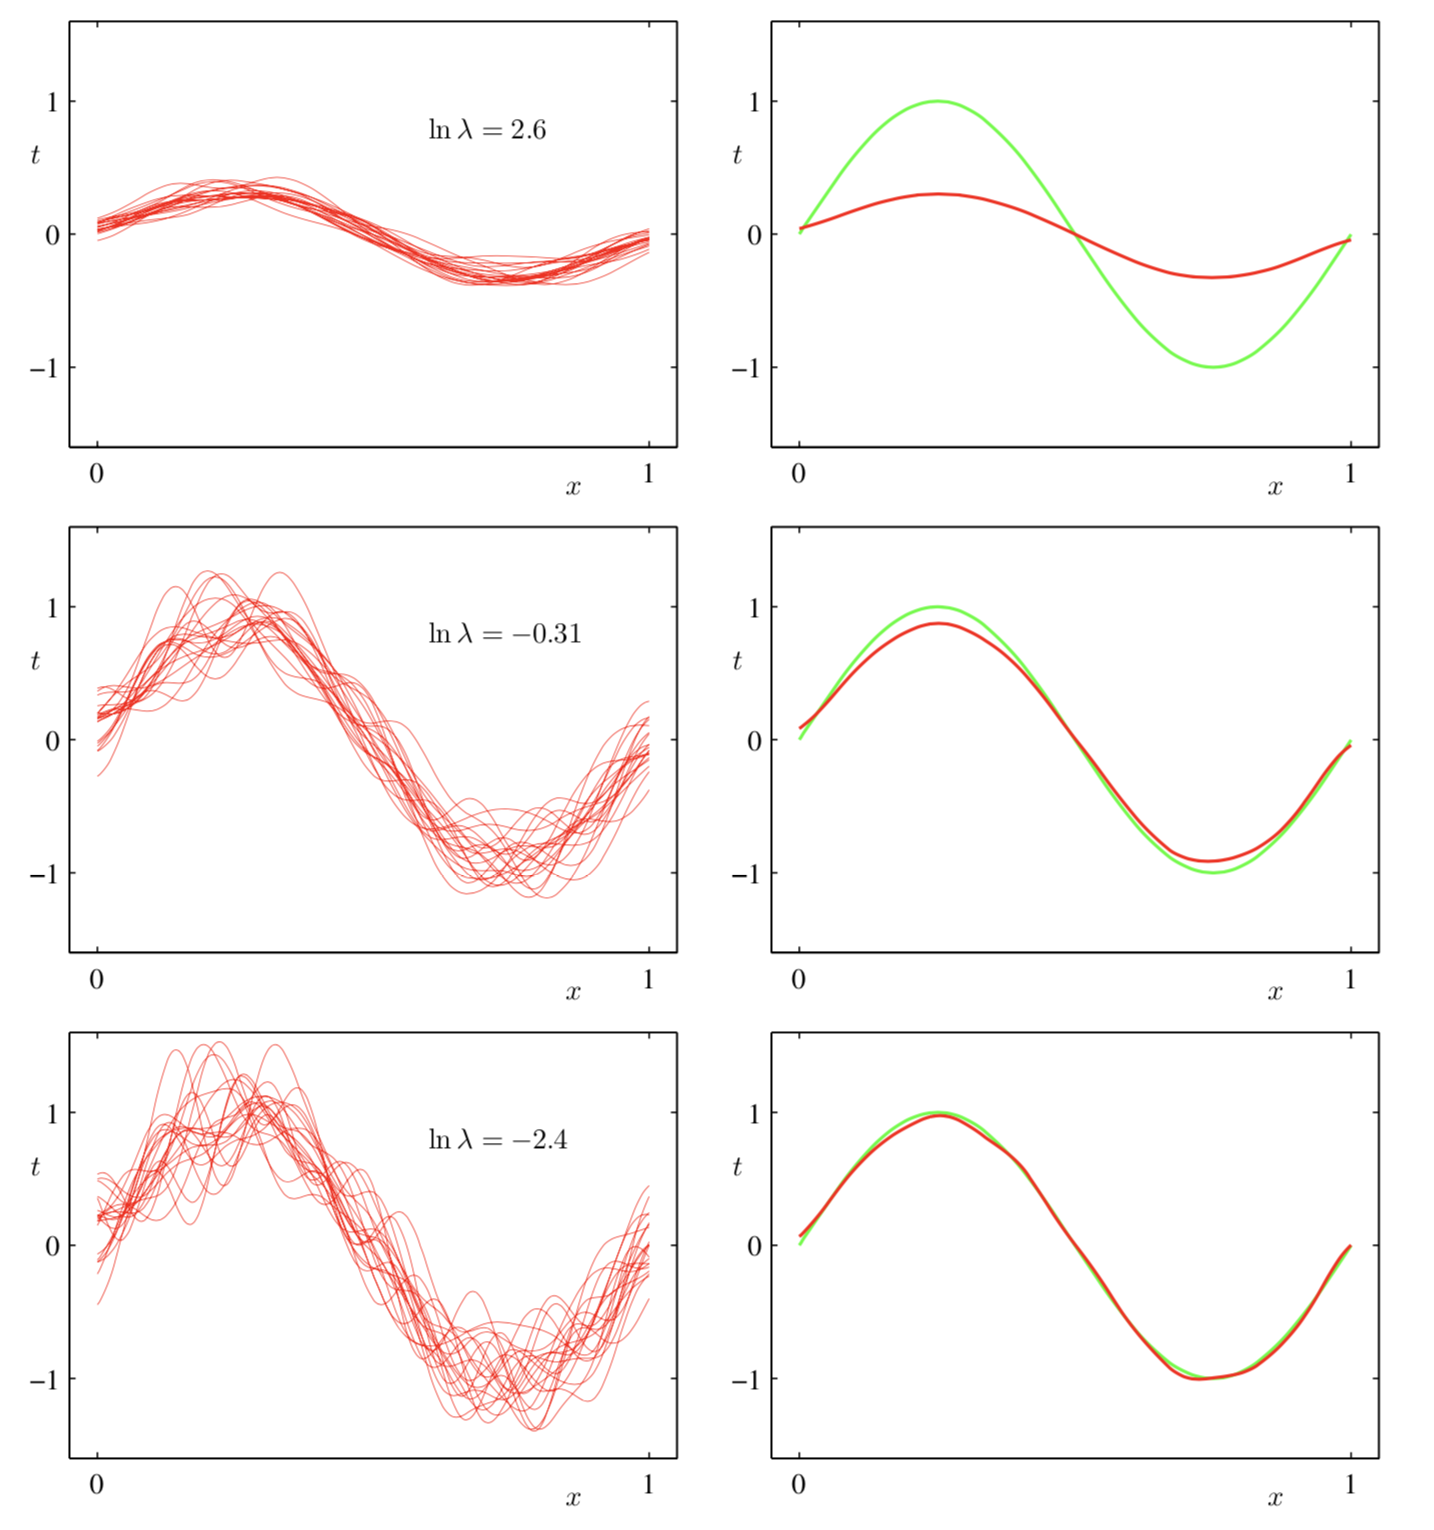
\includegraphics[width=0.4\textwidth]{figures/bias_variance_reg_comp.png}
		\caption{Illustration of dependence of bias and variance on model complexity controlled by $\lambda$. Less complex models (high $\lambda$) tend to have a high bias (be far off the correct distribution) but it is more robust regarding the actual dataset (therefore, a low variance). Decreasing $\lambda$ results in a lower bias, but a high variance as models tend to overfit and are therefore sensitive to the dataset.}
		\label{img:linear_regression_bias_variance_decomp_example}
	\end{figure}
	\item Plotting the terms of the decomposed squared loss function over $\lambda$ gives further insights of the model behavior (see Figure~\ref{img:linear_regression_bias_variance_decomp_error_plot}). For generating such a plot, the integrals are approximated by sums over all data points $x$ as we have a limited number of samples.
	\begin{figure}[ht]
		\centering
		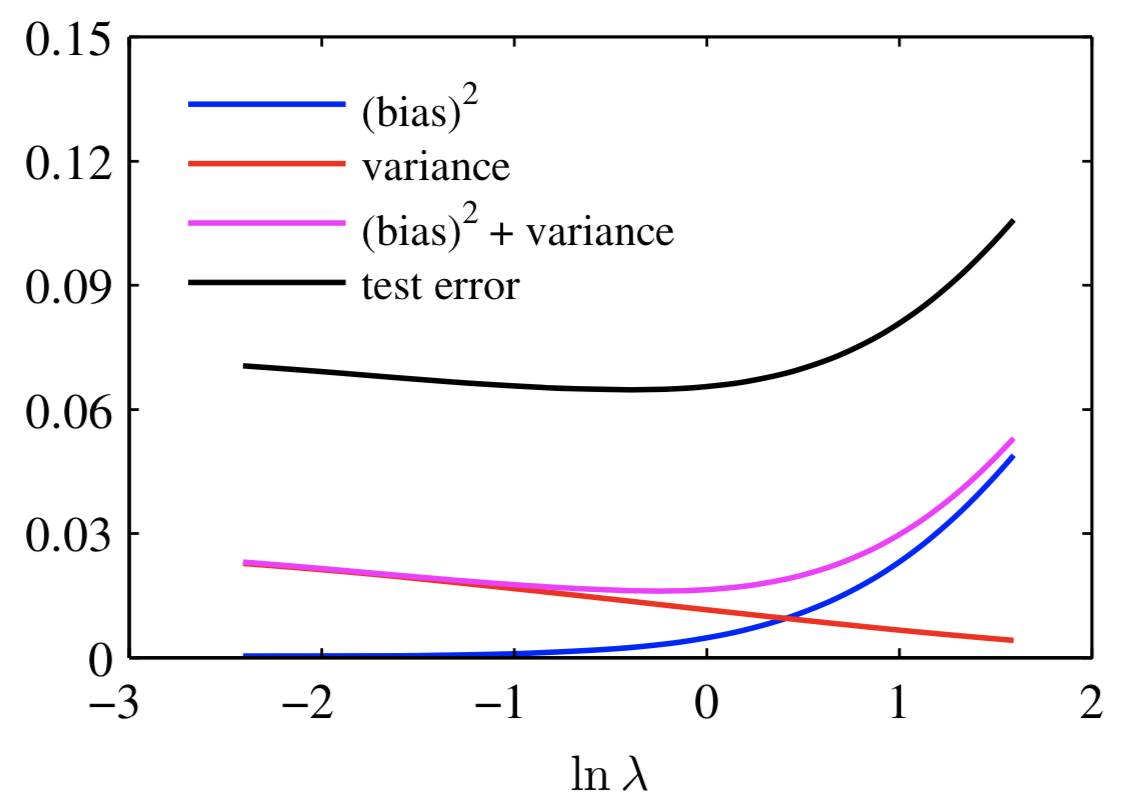
\includegraphics[width=0.4\textwidth]{figures/bias_variance_loss_plot.png}
		\caption{Plot of decomposed loss function for example of Figure~\ref{img:linear_regression_bias_variance_decomp_example}. The goal is to minimize the test error. It is common that this is close to the minimum value of $(\text{bias})^2+\text{variance}$. High variance as on the left indicates overfitting, high bias error on the left shows that the model is underfitting.}
		\label{img:linear_regression_bias_variance_decomp_error_plot}
	\end{figure}
	\item In conclusion, high values of $\lambda$ reduce model complexity, and therefore increase bias loss and leads to underfitting. However, it provides a small variance.\\In contrast, small values of $\lambda$ causes a low bias as the model is quite complex. Still, the variance is high indicating that the model overfits on the small datasets.
	\item The bias-variance decomposition is less practical as it is better to train on one large dataset instead of splitting it into several small ones. Furthermore, this reduces the risk of overfitting for a high model complexity on the data anyways.
\end{itemize}
\subsection{Bayesian Linear Regression}
\begin{itemize}
	\item Determining the suitable model complexity using the training data alone without overfitting
	\item Result is a distribution of $\bm{w}$ instead of single value as in maximum likelihood or posterior
\end{itemize}
\subsubsection{Parameter distribution}
\begin{itemize}
	\item Prior over weights: $p(\bm{w}) = \mathcal{N}\left(\bm{m}_0, \bm{S}_0\right)$
	\item Likelihood: $p\left(t'|\bm{x}', \bm{w}, \beta\right)=\mathcal{N}\left(t'|\bm{\phi}(\bm{x})^T\bm{w}, \beta^{-1}\right)$
	\item Posterior distribution: $p(\bm{w}|\bm{t}, \bm{X}) = \frac{p\left(\bm{t}|\bm{X}, \bm{w}, \beta\right) p\left(\bm{w}\right)}{p\left(\bm{t}|\bm{X}, \beta\right)} = \mathcal{N}\left(\bm{m}_N, \bm{S}_N\right)$, where\\
	$$\bm{S}_N^{-1}=\bm{S}_0^{-1} + \beta \bm{\Phi}^T\bm{\Phi}$$
	$$\bm{m}_N = \bm{S}_N\left(\bm{S}_0^{-1}\bm{m}_0+\beta\bm{\Phi}^T\bm{t}\right)$$
	\item Maximum a posteriori corresponds by $\bm{w}_{\text{MAP}} = \bm{m}_N$
	\item If no prior was given ($\bm{S}_0=\alpha^{-1} \bm{I}$ with $\alpha\to0$) the mean $\bm{m}_N$ reduces to $\bm{w}_{\text{ML}}$
	\item Mostly simpler Gaussian prior used: $p(\bm{w}) = \mathcal{N}\left(\bm{0}, \alpha^{-1}\bm{I}\right)$
	\begin{itemize}
		\item Resulting parameters of posterior: 
		$$\bm{S}_N^{-1}=\alpha^{-1}\bm{I} + \beta \bm{\Phi}^T\bm{\Phi}$$
		$$\bm{m}_N = \beta \bm{S}_N\bm{\Phi}^T\bm{t}$$
		$$p(\bm{w}|\bm{t}, \bm{X})=\frac{1}{\sqrt{\left(2\pi\right)^M |\bm{S}_N|}}\exp\left[-\frac{1}{2}\left(\bm{w}-\bm{m}_N\right)^T \bm{S}_N^{-1} \left(\bm{w}-\bm{m}_N\right)\right]$$
		\item Corresponding log posterior: 
		$$\ln p\left(\bm{w}|\bm{t}, \bm{X}\right) = -\frac{\beta}{2}\sum\limits_{n=1}^{N}\left\{t_n - \bm{w}^T \bm{\phi}\left(\bm{x}_n\right)\right\}^2 - \frac{\alpha}{2}\bm{w}^T \bm{w} + C$$
		\item Thus, maximizing this posterior is equal to having a regularization term with $\lambda=\frac{\alpha}{\beta}$
		\item Infinitely narrow prior by $\alpha\to\infty$ ($\alpha\to0$ seen before ends up in maximum likelihood):
		$$\lim\limits_{\alpha\to\infty} \bm{S}_N = \lim\limits_{\alpha\to\infty} \left(\alpha\bm{I}+\beta \bm{\Phi}^{T}\bm{\Phi}\right)^{-1} = \lim\limits_{\alpha\to\infty} \alpha^{-1}\bm{I} = \bm{0}$$
		$$\lim\limits_{\alpha\to\infty} \bm{m}_N = \lim\limits_{\alpha\to\infty} \beta\left(\alpha\bm{I}+\beta \bm{\Phi}^{T}\bm{\Phi}\right)^{-1}\bm{\Phi}^T \bm{t} = \lim\limits_{\alpha\to\infty} \frac{\beta}{\alpha}\bm{\Phi}^T\bm{t} = \bm{0} = \bm{m}_{0}$$
		\item Infinite data $N\to\infty$:
		$$\lim\limits_{N\to\infty} \bm{S}_N = \lim\limits_{N\to\infty} \left(\alpha\bm{I}+\beta \bm{\Phi}^{T}\bm{\Phi}\right)^{-1} = \lim\limits_{N\to\infty} \left(\bm{\Phi}^{T}\bm{\Phi}\right)^{-1} = \bm{0}$$
		$$\lim\limits_{N\to\infty} \bm{m}_N = \lim\limits_{N\to\infty} \beta\left(\alpha\bm{I}+\beta \bm{\Phi}^{T}\bm{\Phi}\right)^{-1}\bm{\Phi}^T \bm{t} = \lim\limits_{N\to\infty} \left(\bm{\Phi}^T\bm{\Phi}\right)^{-1}\bm{\Phi}^T\bm{t} = \bm{w}_{\text{ML}}$$
		$\Rightarrow$ At infinite data, all approaches agree: $\bm{m}_N = \bm{w}_{\text{ML}} = \bm{w}_{\text{MAP}}$
	\end{itemize}
\end{itemize}

\subsubsection{Sequential Bayesian Learning}
\begin{itemize}
	\item Data is sequences of input $x$ and target $t$
	\item Posterior after $N-1$ data points constitutes the prior for the $N$th data point!
	\item Posterior 1: $p(\bm{w}|x_1,t_1,\alpha,\beta)\propto p(t_1|x_1,\bm{w},\beta)p(\bm{w}|\alpha)$
	\item Posterior 2: $p\left(\bm{w}|(x_1,t_1),(x_2,t_2),\alpha,\beta\right)\propto p(t_2|x_2,\bm{w},\beta)p(\bm{w}|x_1,t_1,\alpha,\beta)$
	\item Posterior narrows down step by step until it gets very certain of the correct estimation 
\end{itemize}
\begin{figure}[ht]
\centering
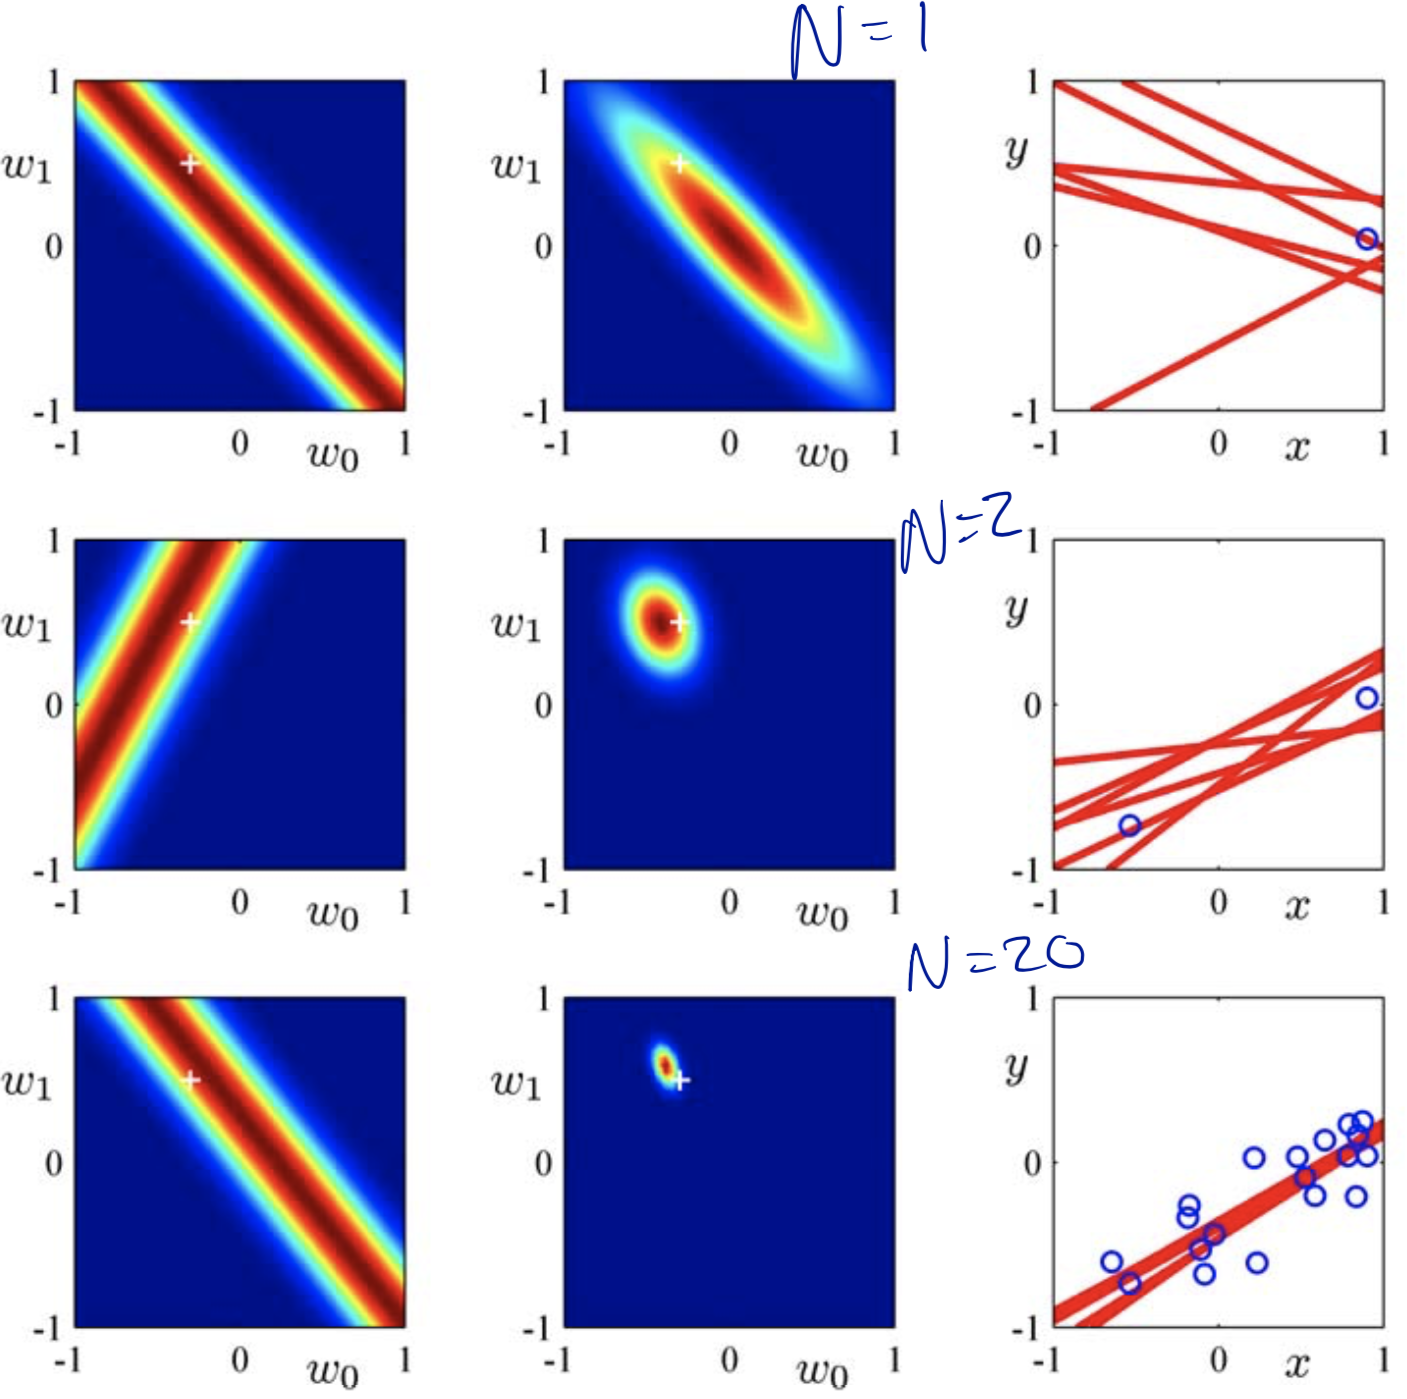
\includegraphics[width=0.5\textwidth]{figures/sequential_bayesian_linear_regression.png}
\caption{Example for Sequential Bayesian Learning on target $t=-0.3+0.5x+\epsilon$. First column: likelihood (not normalized for $\bm{w}$, but for $t_n$!), second column: posterior, third column: sampled weights}
\end{figure}
\subsubsection{Predictive Distribution}
\begin{itemize}
	\item Predictive distribution is defined by ($\bm{\mathtt{t}}$ targets in training set):
	$$p\left(t|x, \bm{\mathtt{t}}, \bm{X}, \alpha, \beta \right) = \int p\left(t|x, \bm{w},\beta\right)p\left(\bm{w}|\bm{\mathtt{t}}, \bm{X}, \alpha, \beta\right)d\bm{w}$$
	where $p\left(t|x, \bm{w},\beta\right) = \mathcal{N}\left(t|y\left(\bm{x},\bm{w}\right), \beta^{-1}\right)$ is the conditional distribution of target variable, and \\$p\left(\bm{w}|\bm{\mathtt{t}}, \bm{X}, \alpha, \beta\right) = \mathcal{N}\left(\bm{w}|\bm{m}_N, \bm{S}_N\right)$ the posterior weight distribution
	\item Predictive distribution is convolution of two Gaussians $\Rightarrow$ $p\left(t|x, \bm{\mathtt{t}}, \bm{X}, \alpha, \beta \right)=\mathcal{N}\left(t|\bm{m}_N^{T}\bm{\phi}(\bm{x}),\sigma_N^2(\bm{x}) \right)$
	where variance $\sigma_N^2(\bm{x})=\frac{1}{\beta} + \bm{\phi}(\bm{x})^T \bm{S}_N \bm{\phi}(\bm{x})$ (first term data noise, second weight uncertainty, which goes to 0 for infinite data $N\to\infty$)
	\item Important points
	\begin{enumerate}
		\item Uncertainty is smaller near training points
		\item Variance/uncertainty decreases with larger $N$
	\end{enumerate}
	\begin{figure}[ht]
		\centering
		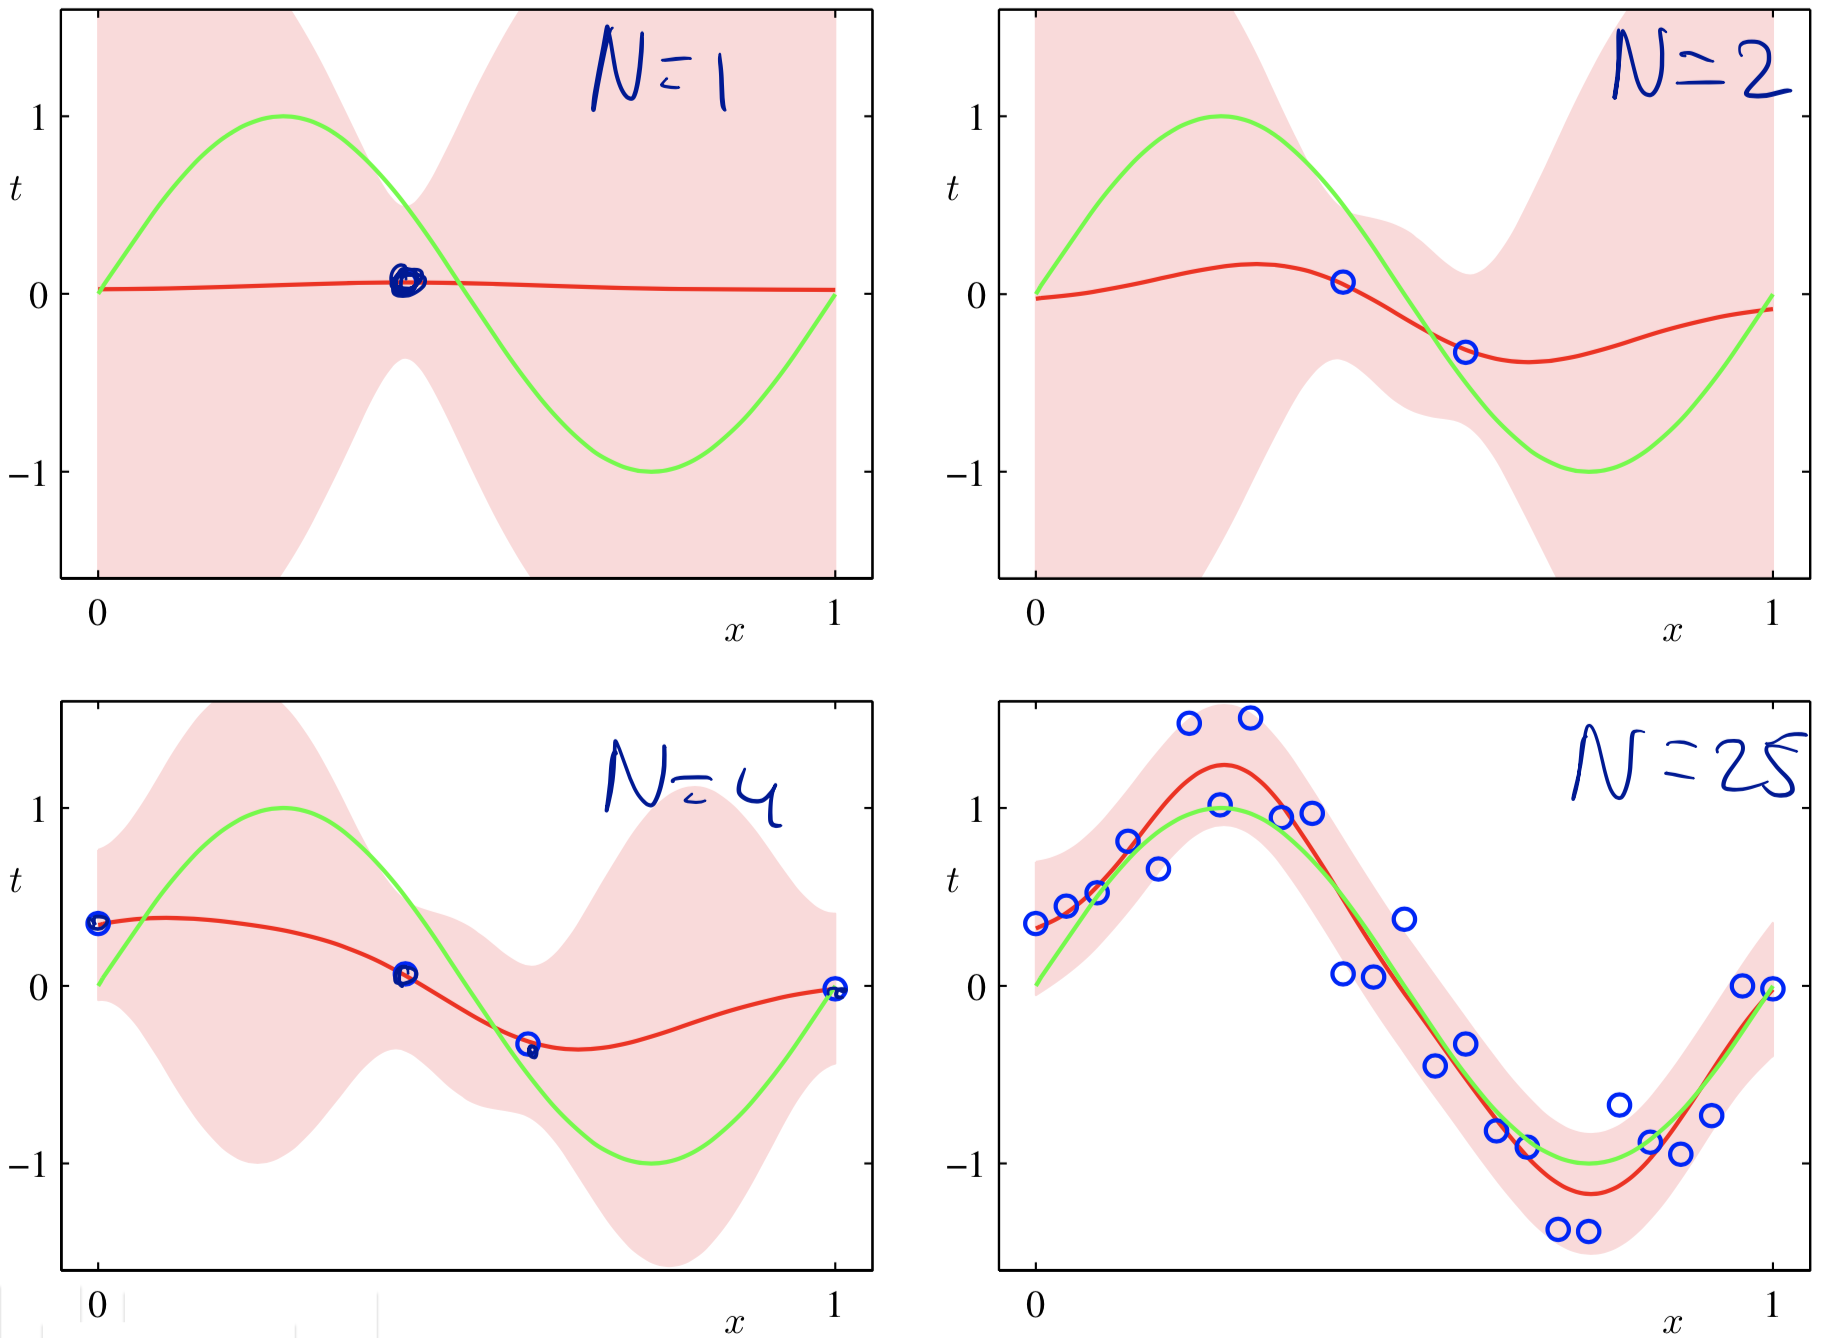
\includegraphics[width=0.5\textwidth]{figures/bayesian_linear_regression_predictive_dist.png}
		\caption{Example for predictive distributions. Green: ground truth data, blue: data points, red line: mean prediction, red area: 1-sigma area}
	\end{figure}
	\item The predictive distribution can be expressed by a \textbf{kernel formulation}:
	\begin{itemize}
		\item The predictive mean is 
		\begin{equation*}
		\begin{split}
			y\left(\bm{x}', \bm{m}_N\right) & = \bm{\phi}^T(\bm{x}') \bm{m}_N = \beta \bm{\phi}^T(\bm{x}')\bm{S}_N \bm{\Phi}^T \bm{t}\\
			& = \beta \bm{\phi}^T(\bm{x}')\bm{S}_N \sum\limits_{n=1}^{N}\bm{\Phi}_{:,n}^T t_n = \beta \sum\limits_{n=1}^{N} \bm{\phi}^T(\bm{x}')\bm{S}_N \bm{\phi}(\bm{x}_n) t_n\\
			& = \sum\limits_{n=1}^{N} k\left(\bm{x}',\bm{x}_n\right) t_n \text{\hspace{5mm} 
				where\hspace{5mm}} k\left(\bm{x}',\bm{x}_n\right)=\beta \bm{\phi}^T(\bm{x}')\bm{S}_N \bm{\phi}(\bm{x}_n)
		\end{split}
		\end{equation*}
		$\Rightarrow$ Prediction is a linear combination of training set target values
		\item Kernel values depend on whole dataset by $\bm{S}_N$
		\item Closer data points to $\bm{x}'$ are given a higher weight than points further removed from $\bm{x}'$
		\item Thus, local evidence is weighted more strongly than distant evidence
		\item Kernel can also express covariance:
		\begin{equation*}
		\begin{split}
		\text{cov}\left[t_1, t_2 | \bm{x}_1, \bm{x}_2\right] & = \text{cov}_{\bm{w}}\left[y(\bm{x}_1, \bm{w}), y(\bm{x}_2, \bm{w})\right] = \text{cov}_{\bm{w}}\left[\bm{\phi}^T(\bm{x}_1)\bm{w}, \bm{w}^T\bm{\phi}(\bm{x}_2)\right]\\
		& = \mathbb{E}_{\bm{w}}\left[\bm{\phi}^T(\bm{x}_1)\bm{w} \bm{w}^T\bm{\phi}(\bm{x}_2)\right] - \mathbb{E}_{\bm{w}}\left[\bm{\phi}^T(\bm{x}_1)\bm{w}\right]\mathbb{E}_{\bm{w}}\left[\bm{w}^T\bm{\phi}(\bm{x}_2)\right]\\
		& = \bm{\phi}^T(\bm{x}_1)\text{cov}\left[\bm{w},\bm{w}\right] \bm{\phi}^T(\bm{x}_2) = \bm{\phi}^T(\bm{x}_1)\bm{S}_N \bm{\phi}^T(\bm{x}_2)\\
		& = \frac{1}{\beta}k\left(\bm{x}_1,\bm{x}_2\right) 
		\end{split}
		\end{equation*}
		\item Based on that, we can see that predictive mean at nearby points will be highly correlated (high values of the kernel), and smaller for distant points
			\begin{figure}[ht]
			\centering
			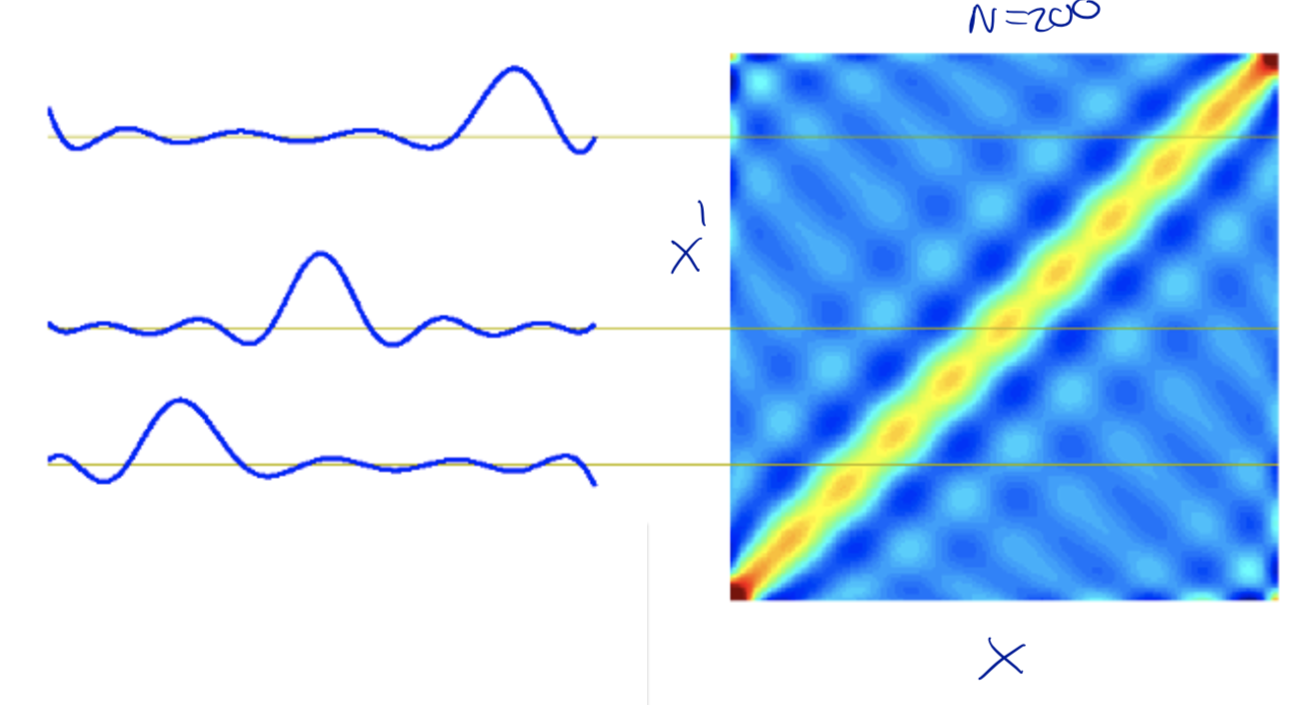
\includegraphics[width=0.5\textwidth]{figures/bayesian_kernel_formulation.png}
			\caption{Right plot: matrix for $(x',x)$ of kernel $k\left(x',x\right)$ for Gaussian basis function. Left plot: slices of this matrix for different values of $x$}
		\end{figure}
		
	\end{itemize}
\end{itemize}
\subsection{Bayesian Model Comparison}
\begin{itemize}
	\item By marginalizing (integrating) over the model parameters instead of making point estimates of their values, models can be directly compared on the training data instead of separate validation data
	\item Compare $L$ models $\left\{\mathcal{M}_i\right\}_{i=1}^{L}$
	\item Probabilities are used to represent uncertainty in the choice of model. 
	\item We express our preference for different models by a prior distribution $p\left(\mathcal{M}_i\right)$, so that the posterior is:
	$$p\left(\mathcal{M}_i|\mathcal{D}\right)\propto p\left(\mathcal{M}_i\right)p\left(\mathcal{D}|\mathcal{M}_i\right)$$
	\item Important term is the \textit{model evidence} $p\left(\mathcal{D}|\mathcal{M}_i\right)$ which updates our preference based on the seen data $\mathcal{D}$. Marginalizes the parameters $\bm{w}$ of a model:
	$$p\left(\mathcal{D}|\mathcal{M}_i\right) = \int p\left(\mathcal{D}|\bm{w}, \mathcal{M}_i\right)p\left(\bm{w}|\mathcal{M}_i\right)d\bm{w}$$
	\begin{itemize}
		\item Can be viewed as the probability that $\mathcal{D}$ is generated by a random sample of $\bm{w}$ from the prior. 
		\item Is also the normalization constant for $p\left(\bm{w}|\mathcal{D}, \mathcal{M}_i\right)$
	\end{itemize}
	\item Two models can be compared by dividing their posteriors:
	$$\frac{p\left(\mathcal{M}_1|\mathcal{D}\right)}{p\left(\mathcal{M}_2|\mathcal{D}\right)} = \frac{p\left(\mathcal{M}_1\right)p\left(\mathcal{D}|\mathcal{M}_1\right)}{p\left(\mathcal{M}_2\right)p\left(\mathcal{D}|\mathcal{M}_2\right)} \text{\hspace{5mm}where\hspace{5mm}} \frac{p\left(\mathcal{D}|\mathcal{M}_1\right)}{p\left(\mathcal{D}|\mathcal{M}_2\right)}\text{ is called \textit{Bayes factor}}$$
	\item The predictive distribution is a weighted mean (based on the model probabilities) of our models:
	$$p\left(t'|\bm{x}',\mathcal{D}\right) = \sum\limits_{i=1}^{L}p\left(t'|\bm{x}', \mathcal{M}_i, \mathcal{D}\right) p\left(\mathcal{M}_i | \mathcal{D}\right)$$
	\item However, a simple approximation is using the single most probable model alone to make prediction $\Rightarrow$ also known as \textit{model selection}
\end{itemize}
\subsubsection{Approximated Model Evidence}
\begin{itemize}
	\item For a single parameter $w$, assume that posterior distribution $p\left(w|\mathcal{D}, \mathcal{M}_i\right)$ is sharply peaked around the most probably value $w_{\text{MAP}}$ with width $\Delta w_{\text{posterior}}$
	\item Further, we assume that also the prior is a flat distribution with width $\Delta w_{\text{prior}}$ so that $p\left(w|\mathcal{M}_i\right) = 1/\Delta w_{\text{prior}}$
	\item Integral of model evidence can be approximated by its maximum value times the width of the peak:
	 $$p\left(\mathcal{D}|\mathcal{M}_i\right) = \int p\left(\mathcal{D}|\bm{w}, \mathcal{M}_i\right)p\left(\bm{w}|\mathcal{M}_i\right)d\bm{w}\simeq p\left(\mathcal{D}|w_{\text{MAP}}, \mathcal{M}_i\right)\frac{\Delta w_{\text{posterior}}}{\Delta w_{\text{prior}}}$$
	 \item Taking the log leads to:
	 $$\ln p\left(\mathcal{D}|\mathcal{M}_i\right) \simeq \underbrace{\ln p\left(\mathcal{D}|w_{\text{MAP}}, \mathcal{M}_i\right)}_{\text{model fit}} + \underbrace{\ln \frac{\Delta w_{\text{posterior}}}{\Delta w_{\text{prior}}}}_{\text{complexity penalty}}$$
	 \item The first term is the likelihood of the data, and therefore describes how good the model fits to the given data (optimal: maximized)
	 \item The second term penalizes model complexity as if $\Delta w_{\text{posterior}} < \Delta w_{\text{prior}}$ (distribution was finely tuned to the data), the term is negative and reduces the model evidence (optimal: minimized)
	 \item Hence, model evidence favors models where we have a trade-off between model fit and complexity
	 \begin{figure}[ht]
	 	\centering
	 	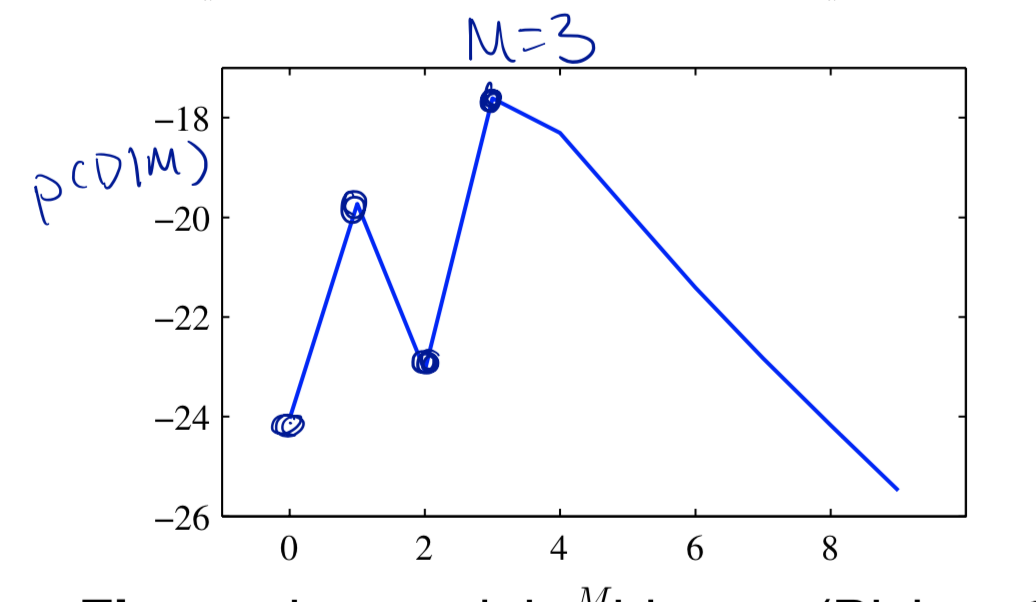
\includegraphics[width=0.5\textwidth]{figures/bayesian_model_comparison_log.png}
	 	\caption{Plotting the curve of $\ln p\left(\mathcal{D}|\mathcal{M}_i\right)$ for different polynomials $M=0,1,...$ for the task of fitting a sine. As the sine is an odd function, polynomials of odd order fit the best (give the most improvement for the model fit). However, increasing the model complexity increases the penalty.}
	 \end{figure}
	 \item For a model with $K$ parameters, we get a similar approximation: 
	 $$\ln p\left(\mathcal{D}|\mathcal{M}_i\right) \simeq \ln p\left(\mathcal{D}|\bm{w}_{\text{MAP}}, \mathcal{M}_i\right) + K \ln \frac{\Delta w_{\text{posterior}}}{\Delta w_{\text{prior}}}$$
	 \item Drawbacks of Bayesian approach:
	 \begin{itemize}
	 	\item Still need to make assumptions about possible models
	 	\item If no model is suitable for the data, the algorithm gives bad estimations
	 	\item Model evidence is sensitive regarding the prior
	 	\item Thus, a small test set is commonly used for Bayesian comparison
	 \end{itemize}
	 \begin{figure}[ht]
	 	\centering
	 	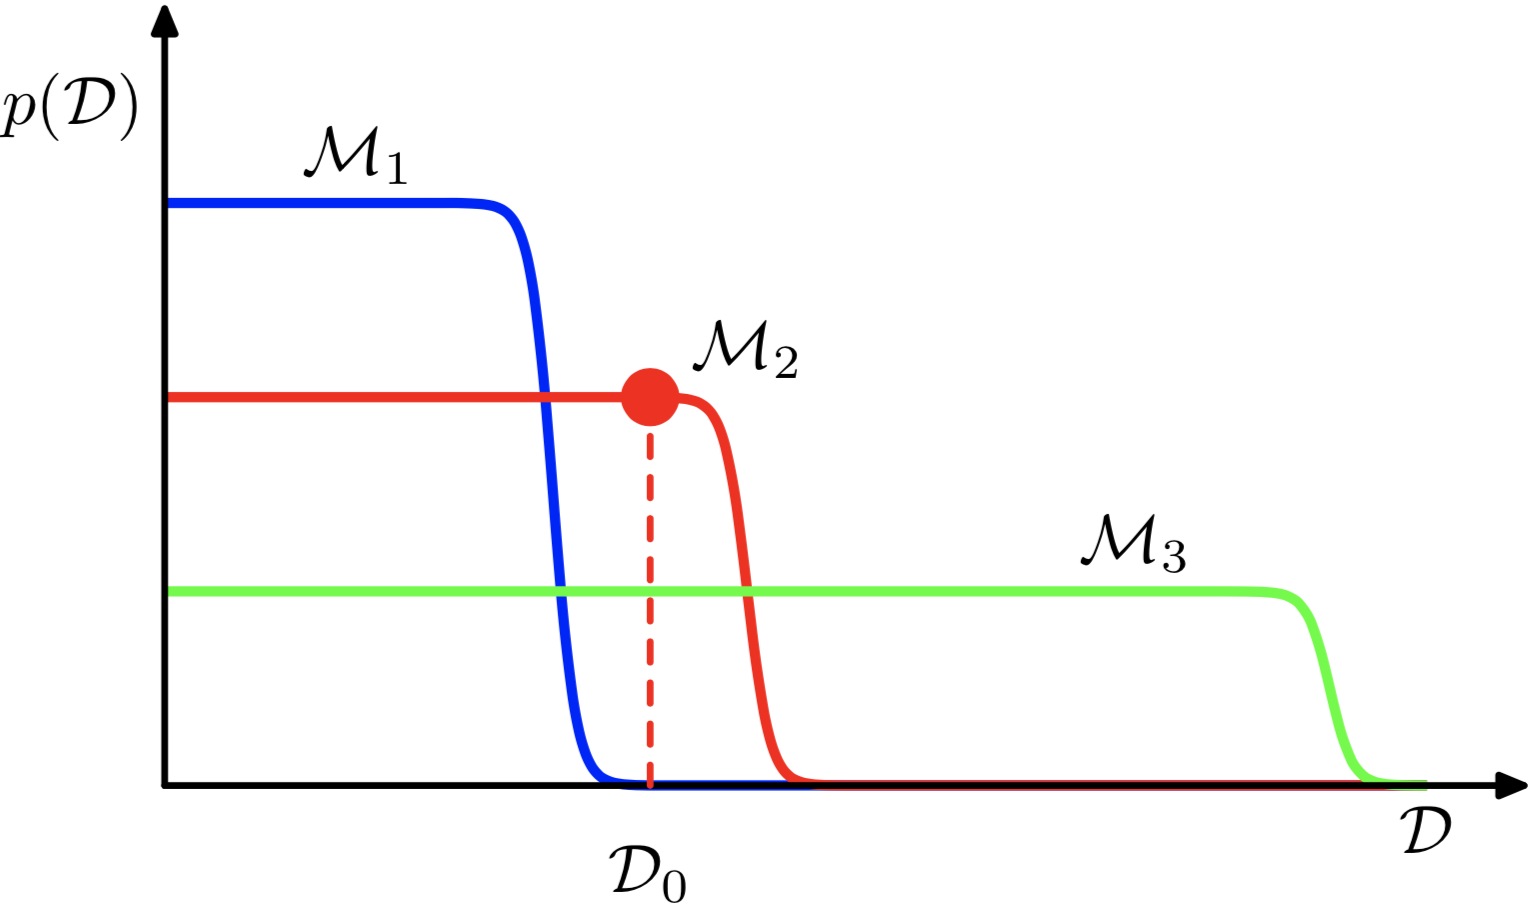
\includegraphics[width=0.4\textwidth]{figures/bayesian_model_comparison.png}
	 	\caption{Illustration of three different models and there corresponding model evidences. Horizontal axis $x$: one dimensional representation of all possible datasets; Vertical axis $y$: probability that these models generate this specific dataset based on their prior distribution of parameters $\bm{w}$. $\mathcal{M}_1$ is the simplest model and is therefore only able to create a small set of different data $\mathcal{D}$. As the probability is normalized over all datasets $\mathcal{D}$, the probability is higher than for more complex models like $\mathcal{M}_2$ and $\mathcal{M}_3$. Given a certain dataset $\mathcal{D}_0$, we choose the model with the highest probability $\Rightarrow$ model which just is enough complex to generate this dataset}
	 \end{figure}
 	
\end{itemize}
\subsubsection{Model Evidence for Linear Basis Models}
\begin{itemize}
	\item In fully Bayesian treatment, we must also consider all hyperparameters:
	\begin{equation*}
		\begin{split}
			p\left(\bm{t}|\bm{X}, \mathcal{M}_i\right) & =\int\int\int p\left(\bm{t}|\bm{X},\bm{w},\beta,\mathcal{M}_i\right)p\left(\bm{w}|\alpha\right)p\left(\alpha, \beta | \mathcal{M}_i\right)d\bm{w}\text{ }d\alpha\text{ }d\beta\\
			& = \int\int \underbrace{p\left(\bm{t}|\bm{X}, \beta, \alpha, \mathcal{M}_i\right)}_{\text{peaked posterior/prior}} \underbrace{p\left(\alpha, \beta | \mathcal{M}_i\right)}_{\text{broad hyperprior}} d\alpha \text{ }d\beta\\
		\end{split}
	\end{equation*}
	\item Note that the hyperprior can again contain new hyperparameters, for which one might have to define a new prior (and so on)
	\item Approximation: take best hyperparameters $\alpha^*$ and $\beta^*$
	$$p\left(\bm{t}|\bm{X}, \mathcal{M}_i\right) = \arg\max_{\alpha, \beta} p\left(\bm{t}|\bm{X}, \beta, \alpha, \mathcal{M}_i\right)$$
	\item Using this approximation, we come to following predictive distribution:
	$$p\left(t'|\bm{x}',\bm{t}, \bm{X}, \mathcal{M}_i^*\right) \approx p\left(t'|\bm{x}',\bm{t}, \bm{X}, \beta^*, \alpha^*, \mathcal{M}_i\right)$$
\end{itemize}
\subsection{Limitations of fixed basis functions}
\textbf{Advantages}
\begin{itemize}
	\item[+] Closed form solution for least-squares problem 
	\item[+] Tractable Bayesian treatment
	\item[+] Nonlinear models mapping input variables to target variables through basis functions
\end{itemize}
\textbf{Limitations}
\begin{itemize}
	\item[-] Assumption: Basis functions $\phi_j(\bm{x})$ are fixed, not learned
	\item[-] \textit{Curse of dimensionality}: to cover growing dimensions $D$ of input vectors, the number of basis functions needs to grow rapidly / exponentially
\end{itemize}